\section{Berechnungen mittels Euler-Lagrange Gleichung}
\subsection{Einleitung}
Einige Probleme lassen sich direkt lösen, indem sie in die hergeleitete Euler-Lagrange-Gleichung eingesetzt werden können. Andere Optimierungsprobleme, bei denen eine Funktion gesucht wird, können gelöst werden, indem sie das Prinzip der Variation von der Euler-Lagrange-Gleichung benutzen. Dazu reicht jedoch nicht mehr ein einfaches einsetzen, sondern es muss eine neue Gleichung hergeleitet werden. Die gesuchte Funktion wird dann gefunden, indem für $g(y)$ und $g'(y)$ konkret $y(x)$ und $y'(x)$ eingesetzt wird. Aber dazu später noch mehr.

\subsection{Beschreibung einer Fata Morgana}
\cite{fataEinleitung}
Bei der physikalischen Betrachtung der Lichtausbreitung geht man davon aus, dass sich Licht in
geradlinig verlaufenden Strahlen fortpflanzt. Das Auge erwartet das Objekt, von dem die Lichtstrahlen
kommen, in rückwärtiger geradliniger Verlängerung der Richtung, welche das Licht beim eintreffen in das Auge besitzt.

Wenn das Licht ein Medium, z.B. mit unterschiedlichen Brechungsindizes durchquert, ändert es seine Richtung wie in \secref{brechungsgesetz} gezeigt. Dies erklärt z.B. die verkürzten Beinen im Schwimmbad.
Eine kompliziertere Situation liegt vor, wenn der Brechungsindex des durch-strahlten Mediums kontinuierlich variiert. 
Dies ist der Fall, wenn die Luft in der Nähe eines stark aufgeheizten Untergrundes erwärmt
wird und infolge der dadurch bewirkten Dichteänderung einen räumlichen variierenden Brechungsindex annimmt. 
Das Licht ändert stetig seine Richtung, dass führt zu Phänomenen wie Luftspiegelungen von Autolichtern oder einer Fata Morgana, an heißen Tagen.

Eintritt in das Auge besitzt. In \figref{Ab:fataEinleitung} wird die Wahrnehmung des Auges und eine Richtungsänderung des Lichtes gezeigt.

\begin{figure}[H]
\begin{center}
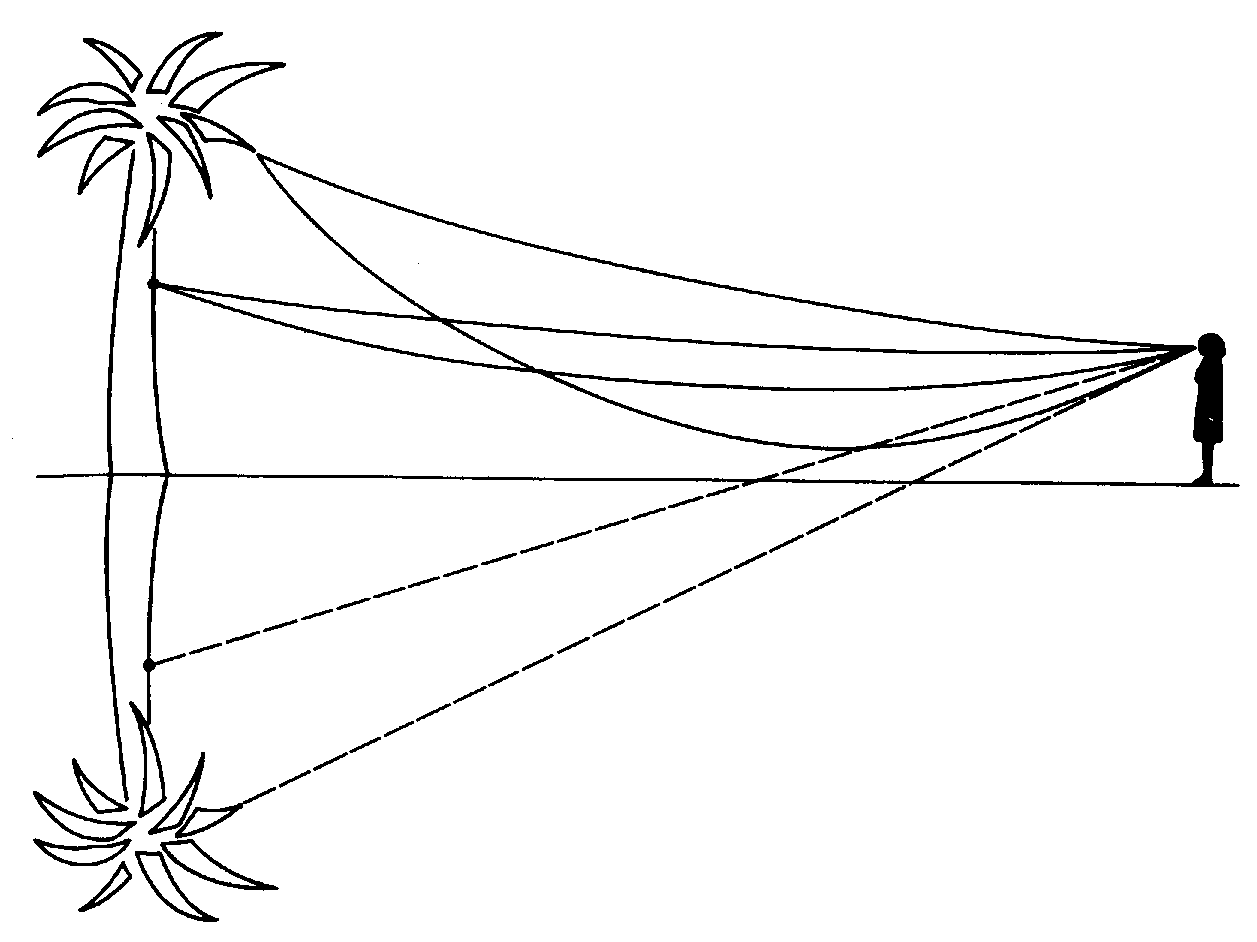
\includegraphics[width=0.5\textwidth]{./picture/FataEinleitung.png}
	\caption{Das Auge interpretiert, dass die Lichtstrahlen mit veränderter Richtung aus der tangentialen Verlängerung kommen und sieht dort das Bild}
	\label{Ab:fataEinleitung}
\end{center}	
\end{figure}


\subsection{Untersuchung der Krümmungs-Eigenschaften bei einer räumlichen Dichteänderung \label{sec:Krümmung}}

Bei einer Fata Morgana hat die Luft eine optische Dichte von $n(x,y)$. 
Dabei bewegt sich das Licht mit der Geschwindigkeit $c/n(x,y)$. 
Die benötigte Zeit, damit das Licht vom Punkt $(x_0, y_0)$ nach $(x_1, y_1)$ braucht,
kann mit dem Kurvenintegral berechnet werden (\eqref{funktionTy}).

\begin{equation}
	T(y) = \int \limits_{x_0}^{x_1} \frac{n(x,y)}{c} \sqrt{1 + y'(x)^2} dx
	\label{funktionTy}
\end{equation}

Wie es bei einem heissen Tag auf einer Strasse oder in einer Wüste zutrifft,
nehmen wir zuerst nur einmal an, dass die optische Dicht nur von $y$ abhängt,
$n(x,y) = g(y)$ und mit zunehmenden $y$ zunimmt.
Dies bedeutet für die Funktion $g(y)$, dass $g(y) > 0$ und $g'(y) > 0 $ ist.

Um dieses Minimalproblem zu lösen, wird die Euler-Lagrange-Gleichung des Variationsproblems aufgestellt (\eqref{krümmung}).

\begin{equation}
	T(y) = \int \limits_{x_0}^{x_1} \frac{g(y)}{c} \sqrt{1 + y'(x)^2} dx = \frac{1}{c} \int \limits_{x_0}^{x_1} g(y) \sqrt{1 + y'(x)^2} dx
	\label{krümmung}
\end{equation}

Der Faktor $\frac{1}{c}$ hat keinen Einfluss auf das Integral und somit auch nicht auf das Variationproblem, deshalb kann er weggelassen werden, um ihn nicht ständig mitschleppen zu müssen.
Es werden nun die Ableitungen der Funktion \ref{funktionRech} gebraucht. Sie sind in \ref{ableitungenLag} aufgeführt.
\begin{align}
	F(x,y,y') &= g(y) \sqrt{1 + y'^2} \label{funktionRech} \\
	\frac{\partial F}{\partial y} &= g'(y) \sqrt{1 + y'^2} \notag \\
	\frac{\partial F}{\partial y'} &= g(y) \frac{y'}{\sqrt{1 + y'^2}}
	\label{ableitungenLag}
\end{align}

Für die Euler-Lagrange-Gleichung muss man im zweiten Ausdruck für $y$ und $y'$ die Funktionen $y(x)$ 
sowie $y'(x)$ einsetzen und nach $\frac{d}{dx}$ ableiten, (\eqref{lagrange1}).

\begin{align}
	\frac{d}{dx} \frac{\partial F}{\partial y'} &= \frac{d}{dx} (g(y(x)) \frac{y'(x)}{\sqrt{1 + y'(x)^2}}) \notag \\ 
	&= g'(y(x)) \frac{y'(x)^2}{\sqrt{1 + y'(x)^2}} + g(y(x)) \frac{y''(x)}{\sqrt{1 + y'(x)^2}}
	 - g'(y(x)) \frac{y'(x)^2 y''(x)}{(1 + y'(x))^\frac{3}{2}} 
	 \label{lagrange1}
\end{align}

Auch im zweiten Term der Euler-Lagrange-Gleichung wird für $y'$ $y'(x)$ eingesetzt. Es ergibt sich \eqref{lagrange2}
\begin{align}
	0 = \frac{d}{dx} \frac{\partial F}{\partial y'} - \frac{\partial F}{\partial y}
	= g'(y(x)) \frac{y'(x)^2}{\sqrt{1 + y'(x)^2}} + g(y(x)) \frac{y''(x)}{\sqrt{1 + y'(x)^2}} \notag \\
	- g'(y(x)) \frac{y'(x)^2 y''(x)}{(1 + y'(x)^2)^\frac{3}{2}}  - g'(y(x)) \sqrt{1 + y'(x)^2}
	\label{lagrange2}
\end{align}

Da $\sqrt{1 + y'(x)^2} > 0$ und somit nicht gleich Null ist kann die Gleichung mit $\sqrt{1 + y'(x)^2}$  multipliziert werden um einen einfacheren Ausdruck zu bekommen, (\eqref{lagrange3}).

\begin{align}
	0 = g'(y(x)) y'(x)^2 + g(y(x)) y''(x) - g'(y(x)) \frac{y'(x)^2 y''(x)}{1 + y'(x)^2} - g'(y(x)) (1 + y'(x)^2)
	\label{lagrange3}
\end{align}

Auch $g(y(x))$ ist nicht gleich Null, da nach eingangs erfolgter Definition $g(y(x)) > 0$, eine Division mit $g(y(x))$ ist somit zulässig, (\eqref{lagrange4}).

\begin{align}
	\frac{g'(y(x))}{g(y(x))} (1 + y'(x)^2) - \frac{g'(y(x))}{g(y(x))} y'(x)^2 &=  y''(x) - \frac{y'(x)^2 y''(x)}{1 + y'(x)^2} \notag \\
	\frac{g'(y(x))}{g(y(x))} (1 + y'(x)^2 - y'(x)^2) &= \frac{\left(1 + y'(x)^2 \right)y''(x) - y'(x)^2 y''(x)}{1 + y'(x)^2} \notag \\
	\frac{g'(y(x))}{g(y(x))} = \frac{y''(x) + y'(x)^2 y''(x) - y'(x)^2 y''(x)}{1 + y'(x)^2} &= \frac{y''(x)}{1 + y'(x)^2}\notag \\
	\frac{g'(y(x))}{g(y(x))} &= \frac{y''(x)}{1 + y'(x)^2}
	\label{lagrange4}
\end{align}


\eqref{lagrange4} kann jetzt auf ihre Eigenschaften bezüglich der Krümmung untersucht werden. Gemäss den Definitionen von ganz am Anfang ist die linke Seite positiv. 
Der Nenner der rechte Seite ist ebenfalls positiv, daraus resultiert, dass der Zähler der rechten Seite ebenfalls positiv sein muss, (\eqref{krümmungAuswertung}).

\begin{align}
	\frac{g'(y(x))}{g(y(x))} > 0 \qquad \wedge \qquad (1 + y'(x)^2) > 0 \qquad \Rightarrow \qquad y''(x) > 0
	\label{krümmungAuswertung}
\end{align}

Da die zweite Ableitung positiv ist, muss die Funktion des Lichtstrahles konvex sein.
Dies bedeutet, dass der Lichtstrahl sich über dem Boden nach oben biegt, ganz egal wie die Funktion von $g(x)$ aussieht, solange sie monoton steigend ist.
Daraus kann die verallgemeinerte Schlussfolgerung gezogen werden, dass der Lichtstrahl konkav sein muss, wenn die Funktion $g(x)$ monoton fallend ist.
\begin{hilfssatz}
Ein Lichtstrahl wird in einem inhomogenen Medium in Richtung höherer Dichte gekrümmt, verhält sich die Dichteänderung monoton fallend oder steigend, nimmt der Lichtstrahl eine konvexe oder konkave Kurvenform an.
\index{Krümmung von Lichtstrahlen}
\end{hilfssatz}

\subsubsection{Technische Anwendung dieser Erkenntnis}
In einem Lichtwellenleiter wird dieses Phänomen ausgenutzt, 
indem  die  optische  Dichte  eines  zylindrischen
Lichtwellenleiters  von  der Achse zum Mantel hin abnimmt.
So werden die Lichtstrahlen immer vom Mantel weggekrümmt 
und das Licht  bleibt im Leiter gefangen.

\begin{figure}[H]
\begin{center}
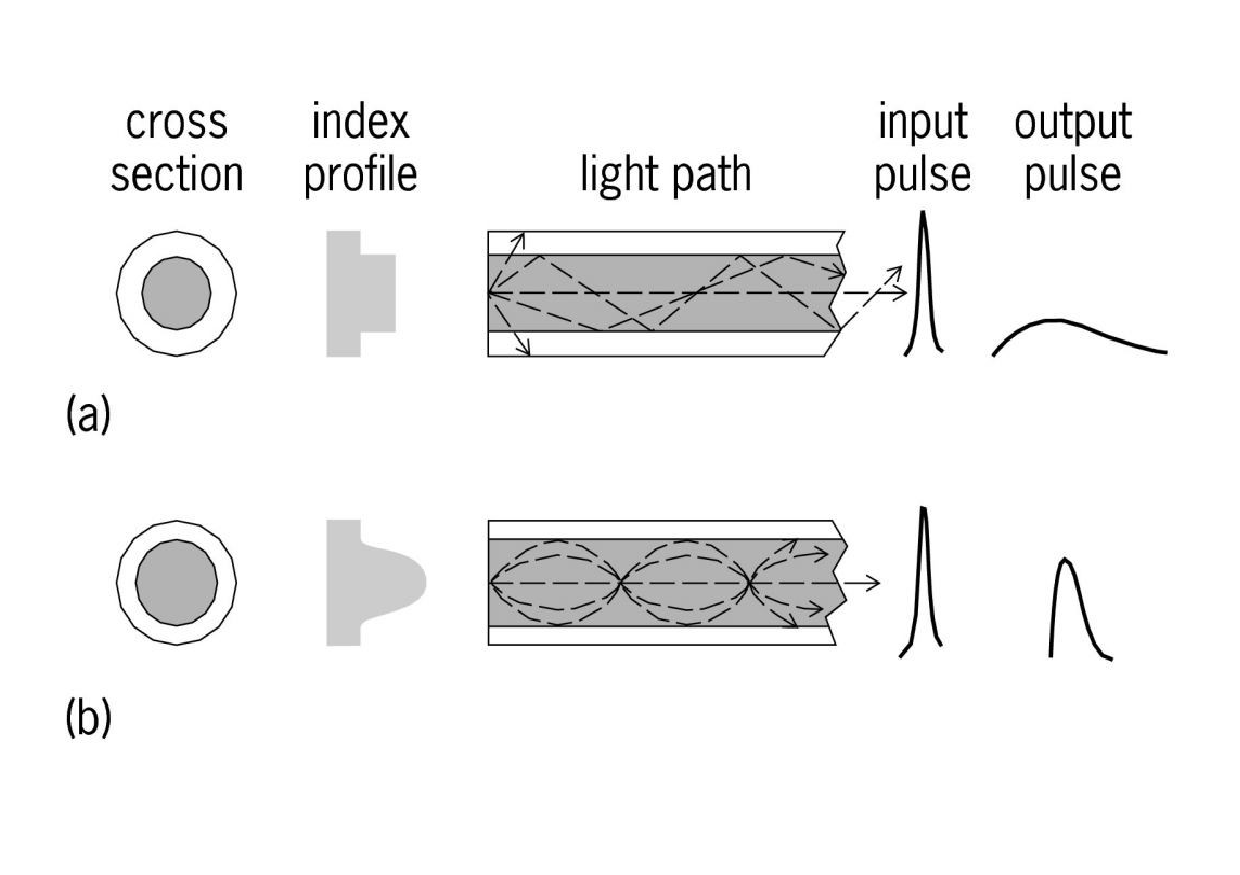
\includegraphics[width=0.5\textwidth]{./picture/Lichtwellenleiter.pdf}
	\caption{Lichtwellenleiter mit einer Sprunghaften Änderung der optischen Dichte erzeugt einen am Übergang Reflektierenden Lichtweg. 
	Lichtwellenleiter mit einer stetig ändernden optischer Dichte erzeugt einen krümmenden Lichtstrahl.}
	\label{Ab:fataEinleitung}
\end{center}	
\end{figure}

\subsection{Berechnung der Differentialgleichung einer Fata Morgana}

Für die gesuchte Differentialgleichung der Fata Morgana nehmen wir wie bei der Krümung an das die optische Dichtung nur $y$ abhängt. Durch die geringe Krümmung der Erde kann die $x$ Richtung vernachlässigt werden.
$n(x,y) = g(y)$ und mit zunehmenden $y$ zunimmt. Dies bedeutet wie für die Funktion $g(y)$ wie in \secref{sec:Krümmung}, dass $g(y) > 0$ und $g'(y) > 0 $ ist.

Die Euler-Lagrange-Gleichung wird gleich wie in \secref{sec:Krümmung} berechnet. Bei \eqref{lagrange4} wird weiter gerechnet. In (\eqref{diffgleichung1}) werden alle Terme auf die linke Seite genommen.
\begin{align}
	g(y(x)\cdot y''(x)-g'(y(x)\cdot y'(x)^2 - g'(y(x)) =0 
	\label{diffgleichung1}
\end{align}

$g(y(x))$ ist unsere Funktion des Brechungsindex $n(y)$. Mit dieser Substitution ergibt sich differentiationsgleichung (\eqref{diffgleichung2}).
\begin{align}
	n\cdot y''-n'\cdot (y')^2 - n' =0 
	\label{diffgleichung2}
\end{align}

In \secref{sec:Krümmung} war die anfangs definiert worden das die Dichte ab dem Boden richtung $y$ zunimmt weil die Temperatur über dem Boden von dem heissen Untergrund mehr erhitzt ist als in höheren Lagen. Wird jetzt diese Temperaturabnahme als linear angenommen, gilt \eqref{einsetzGl1} und deren Ableitung (\eqref{einsetzGl2}).
\begin{align}
	n(y)&=my+b \label{einsetzGl1} \\
	n'(y)&=m \label{einsetzGl2}
\end{align}

Um die Differentiation Gleichung zu lösen, kann für $y$ eine hyperbolische Funktion \cite{cosh} gewählt werden (\eqref{hyperFunk}).
\begin{align}
	y&=A\cdot\cosh(Bx+C)+D \label{hyperFunk} \\
	y'&= A\cdot B\cdot sinh(B x + C) \label{hyperFunkDx} \\
	y''&= A\cdot B^2\cdot cosh(B x + C) \label{hyperFunkD2x}
\end{align}


\subsubsection{Eine Beispiel Aufgabe}

Folgende Annahmen gelten:

%\begin{tabularx}{\textwidth}{XX}
%	$y_0=y_1=2 m$ & Augenhöhe und Startpunkt \\
%	$-x_0=x_1 = 200m$ & Temperatur Luft auf Augenhöhe \\
%	$T_A=333.15 K$ & Temperatur des Aspalt \\
%	$T_L=293.15 K$ & Temperatur Luft auf Augenhöhe \\
%	$-x_0=x_1 = 200m$ & Temperatur Luft auf Augenhöhe \\
%\end{tabularx}

\begin{align}
	y_0&=y_1=2 m & \text{Augenhöhe und Startpunkt} \notag \\
	-x_0&=x_1 = 200m \qquad& \text{Distanz zum Nullpunkt des Kordinatensystems} \notag \\
	T_A&=333.15 K & \text{Temperatur des Aspalt}  \notag \\
	T_L&=293.15 K & \text{Temperatur Luft auf Augenhöhe}  \notag \\
\end{align}

Daraus ergeben sich mit \eqref{brechTemp} eine Funktion für den Brechungsindex von Luft in abhängigkeit von Temperatur.
\begin{align}
	n=1+0.000293\frac{T_0}{T}
	\label{brechTemp}
\end{align}
Daraus ergeben sich die werte in \eqref{nParam} für unsere lineare gleichung $n(y)=my+b$
\begin{align}
	y&=y_0=y_1 \notag \\
	b&=n_A=1+0.000293\frac{273.15 K}{333.15 K} = 1.00024 \notag \\
	n_L&=1+0.000293\frac{273.15 K}{293.15 K} = 1.00027 \notag \\
	m&=\frac{\delta n}{y}=\frac{n_L-n_A}{y}=1.64*10^{-5} \notag \\
	n(y)&=my+b=1.64*10^{-5}y +1.00024
	\label{nParam}
\end{align}

Als erstes die allgemeine Form mit einsetzen von $n,n',y',y''$ (\eqref{HauptGl}).
\begin{align}
	(my_0+b)A\cdot B^2\cdot cosh(B x_0 + C)-m (A\cdot B\cdot sinh(B x_0 + C))^2-m &= 0\notag \\
	(my_1+b)A\cdot B^2\cdot cosh(B x_1 + C)-m (A\cdot B\cdot sinh(B x_1 + C))^2-m &=0 \label{HauptGl}
\end{align}

Da wir $y_0$ und $y_1$ gleich haben und $-x_0=x_1$ eine Achsenspieglung und Cosinus Hyperbolicus Funktion eine gerade Funktion ist lässt sich (\eqref{HauptGl}) vereinfachen (\eqref{glvereinfacht}). Dabei wird $C$ weggelassen.
\begin{align}
	(my_0+b)A\cdot B^2\cdot cosh(B x_0 )-m (A\cdot B\cdot sinh(B x_0 ))^2-m &= 0\notag \\
	(my_1+b)A\cdot B^2\cdot cosh(B x_1 )-m (A\cdot B\cdot sinh(B x_1 ))^2-m &=0 \label{glvereinfacht}
\end{align}

